\documentclass{article}
\usepackage{amsmath}
\usepackage{amssymb}
\usepackage{graphicx}
\usepackage{tikz,pgfplots}
\usepackage[utf8]{inputenc}
\pgfplotsset{compat=1.11}

%Primero será necesario inicializar el documento%
%Inicio documento%
\begin{document}
%Ahora se comenzara a hacer la portada para comenzar con el trabajo%
%Inicio Portada%
    \begin{titlepage}
        %Centraremos el texto para comenzar%
        \centering
        %Fotografia del escudo de la escuela%
        {\includegraphics[width=0.2\textwidth]{logo.png} \par}
        %Texto de la portada%
        {\bfseries\LARGE\textit{Universidad Nacional Autónoma de México}\par}
        %Vspace sera el espacio que existe entre un parrafo y el siguiente%
        \vspace{1cm}

        {\scshape\Large Facultad de Estudios Superiores Acatlán \par}
        \vspace{3cm}

        {\scshape\Huge Ejercicio 3: Aún r}
        \vspace{3cm}

        {\slshape\Large Materia: Métodos Numéricos $1$ \par}
        \vfill

        {\Large Autor: Díaz Valdez Fidel Gilberto \par}
        {\Large Número de cuenta: 320324280 \par}

        \vfill
        {\Large Septiembre 2023 \par}

    \end{titlepage}

\section{Propósito}
Hacer uso del método numérico de Newton-Raphson para aplicarlo en la problemática a resolver para así encontrar una solución satisfactoria al problema además de ganar soltura y experiencia tanto en la utilización de este método, como en la aplicación de otras dependiendo de lo que se requiera y las herramientas que se dispongan. 

\section{Instrucciones}
Según la ecuación de Van der Waals para algún gas real encontrar el valor de $V$. 

El gas en cuesitón es dimetilamina y la ecuación la siguiente:
$$ (P+\frac{a}{V^2})(V-b)=RT $$

Los datos proporcionados:
\begin{itemize}
    \item $P$ = Presión en $atm$ (atmosférica) = $50 atm$
    \item $T$ = Temperatura en $K$ (Kelvin) = $75$ $C$º
    \item $R$ = $0.08205 atm-L/(gmolK)$
    \item $V$ = Volumen molar del gas en $L/mol$
    \item $a$ = Constante del gas dimetilamina = $37.49$
    \item $b$ = Constante del gas dimetilamina = $0.197$
\end{itemize}

\section{Fórmula}
El siguiente paso es sustituir los valores que nos proporcionan en la misma ecuación.

Pero antes de hacer esto es necesario pasar la temperatura a Kelvin ya que se nos fue proporcionada en Celsius.

La fórmula es esta: $75$Cº$+243.15K= 348.15K$


El resultado de sustituir los datos es:
$$ (50+\frac{37.49}{V^2})(V-0.197)=(0.08205)(348.15) $$
Lo que nosotros realmente necesitamos es el valor de $V$ que satisfaga la ecuación y esto se podría hacer al resolver la ecuación pero si suponemos el coso en donde es muy complicado resolverla como normalmente lo hacemos por medio de algebra, aquí es donde entra el método de Newton-Raphson.

Lo que realmente necesitamos es que se satisfaga la ecuación por lo que primero la igualamos a cero teniendo como resultado lo siguiente:
$$ (50+\frac{37.49}{V^2})(V-0.197)-28.5657075=0$$
Como mencione anteriormente, sería necesario encontrar el valor de $V$ y esto se podría realizar al solo despejar, es decir, encontrar el valor de $V$ que cumple que realizando las operaciones correspondientes con los datos proporcionados se cumpla que el resultado final de las operaciones es 0.

Es decir buscar la $V$ que haga que el resultado sea cero, casi como si se tratará de una función, pero como ya mencionamos buscamos hacer uso del método de Newton-Raphson por lo que necesitamos una función que evaluar en diferentes puntos hasta encontrar la $V$ que nos arroje una raíz, es decir, que haga que el resultado de la ecuación sea 0.

Haciendo este análisis y teniendo la ecuación igualada a cero podemos afirmar que la función que utilizaremos para encontrar el valor de $V$ que nos devuelve una raíz es:
$$f(x) = (50+\frac{37.49}{x^2})(x-0.197)-28.5657075$$


Teniendo la función a utilizar para el método ya estamos en condiciones de graficar.

\section{Gráfica}
 \begin{figure}[h]
    \centering
    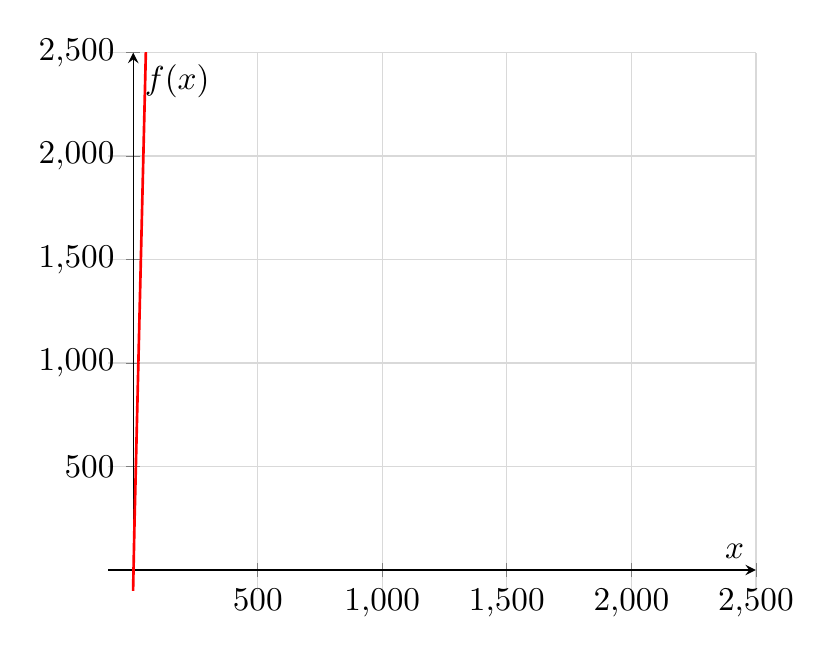
\begin{tikzpicture}[scale=1.2]
        \begin{axis}[
          axis lines= middle,
            xlabel=$x$,
            ylabel=$f(x)$,
            xmin=-100, xmax=2500,   % Amplía los límites del eje x
            ymin=-100, ymax=2500,     % Ajusta los límites del eje y según tus datos
            grid=major,  % Activa la cuadrícula
            grid style={gray!30},  % Estilo de la cuadrícula
            ]
            \addplot[domain=-20:2500, samples=400, color=red, thick]{(50+(37.49/x^2))*(x-0.197)-28.57};
        \end{axis}
    \end{tikzpicture}
    
 \end{figure}

Así es como se comporta la función de manera general, agrande la escala para poder ser capaces de apreciar como se comporta ya que muy de cerca tiene parecido a una simple recta. 
La funcion más de cerca para apreciar su raíz es la siguiente:
        
\begin{figure}[h]
    \centering
    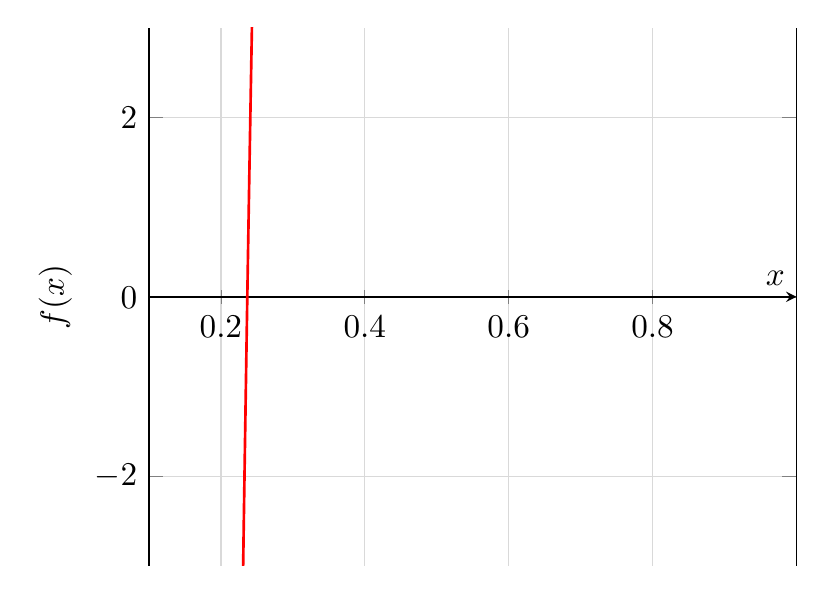
\begin{tikzpicture}[scale=1.2]
        \begin{axis}[
            axis x line = center,
            xlabel=$x$,
            ylabel=$f(x)$,
            xmin=0.1, xmax=1,   % Amplía los límites del eje x
            ymin=-3, ymax=3,     % Ajusta los límites del eje y según tus datos
            grid=major,  % Activa la cuadrícula
            grid style={gray!30},  % Estilo de la cuadrícula  % Altura de la gráfica
            ]
            \addplot[domain=0.1:1, samples=1000, color=red, thick]{(50+(37.49/x^2))*(x-0.197)-28.57};
        \end{axis}
    \end{tikzpicture}
\end{figure}

\section{Intervalo de solución}
Como se puede ver en la segunda grafica la raíz se encuentra entre $0.2$ y $0.4$ por lo que ese sera el intervalo que escogeremos para encontrar la raíz: $[0.2, 0.4]$


\begin{figure}[h]
    \centering
    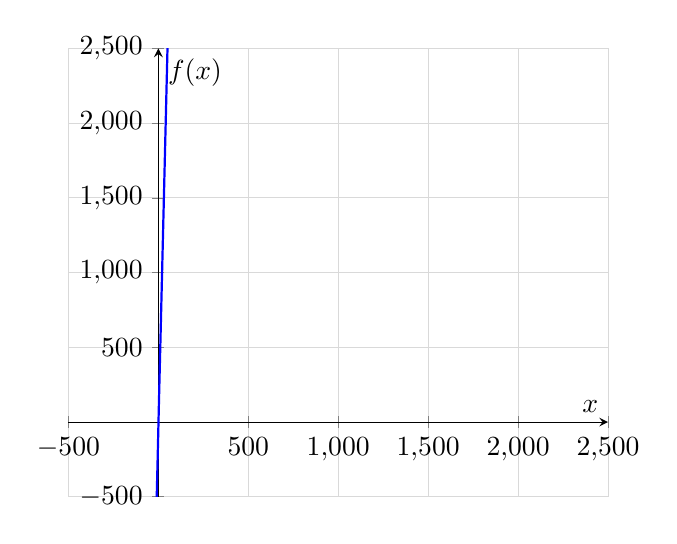
\begin{tikzpicture}
        \begin{axis}[
            axis lines=middle,
            xlabel=$x$,
            ylabel=$f(x)$,
            xmin=-500, xmax=2500,   % Límites del eje x
            ymin=-500, ymax=2500,   % Límites del eje y
            xtick={-500,0,500,1000,1500,2000,2500}, % Marcas en el eje x
            ytick={-500,0,500,1000,1500,2000,2500}, % Marcas en el eje y
            grid=major,  % Activa la cuadrícula
            grid style={gray!30},  % Estilo de la cuadrícula
        ]
        % Función a graficar
        \addplot[domain=-500:2500, samples=400, color=blue, thick]{(50 + (37.49/x^2))*(x - 0.197) - 28.5657075};
        \end{axis}
    \end{tikzpicture}
\end{figure}

\begin{figure}[h]
    \centering
    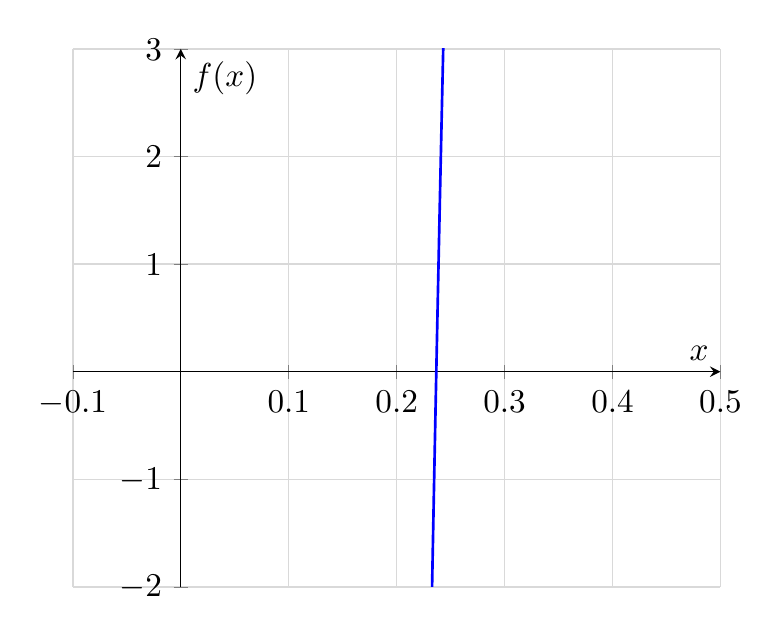
\begin{tikzpicture}[scale=1.2]
        \begin{axis}[
            axis lines=middle,
            xlabel=$x$,
            ylabel=$f(x)$,
            xmin=-0.1, xmax=0.5,   % Límites del eje x
            ymin=-2, ymax=3,   % Límites del eje y
            xtick={-0.1,0, 0.1, 0.2, 0.3, 0.4, 0.5}, % Marcas en el eje x
            ytick={-2, -1, 0, 1, 2,3}, % Marcas en el eje y
            grid=major,  % Activa la cuadrícula
            grid style={gray!30},  % Estilo de la cuadrícula
        ]
        % Función a graficar
        \addplot[domain=0.1:0.3, samples=1000, color=blue, thick]{(50 + (37.49/x^2))*(x - 0.197) - 28.5657075};
        \end{axis}
    \end{tikzpicture}
\end{figure}

\end{document}
%Fin Documento%